
\begin{center}
Code at \url{https://github.com/cedrict/fieldstone/tree/master/python_codes/fieldstone_85}
\end{center}

\par\noindent\rule{\textwidth}{0.4pt}

{\sl This stone was developed in collaboration with Rens Elbertsen, Bart Root, and Ross Maguire}. 
\index{contributors}{R. Elbertsen}
\index{contributors}{B. Root}
\index{contributors}{R. Maguire}

\par\noindent\rule{\textwidth}{0.4pt}
%%%%%%%%%%%%%%%%%%%%%%%%%%%%%%%%%%%%%%%%%%%%%%%%%%%%%%%%%%%%%%%%%%%%%%%%%%%%%%%%%%%%%%%%%%%%%%

\vspace{1cm}

\index{general}{S20RTS}
\index{general}{S40RTS}


The S20RTS \cite{rivw99} and S40RTS \cite{ridv11} are commonly used shear-velocity models for the mantle.
The dataset are widely available (one, in specfem, in aspect, ...) and come in the form of two 
files {\sl S20RTS.sph} and {\sl S40RTS.sph}. 
Each file has a 1 line header, and the first number on this line indicates the maximum degree number $l$ 
(20 or 40, then). The rest of these files consists of many rows and colums of numbers.

Let us recall that for a given value of the degree $l$ the order $m$ is such that $-l \le m \le +l$, i.e. 
there are $2l+1$ values of $m$ for a single value of $l$. Concretely:
\begin{itemize}
\item $l=0$, $m=1$ 
\item $l=1$, $m=-1,0,+1$ 
\item $l=2$, $m=-2,-1,0,+1,+2$ 
\end{itemize}

\begin{center}
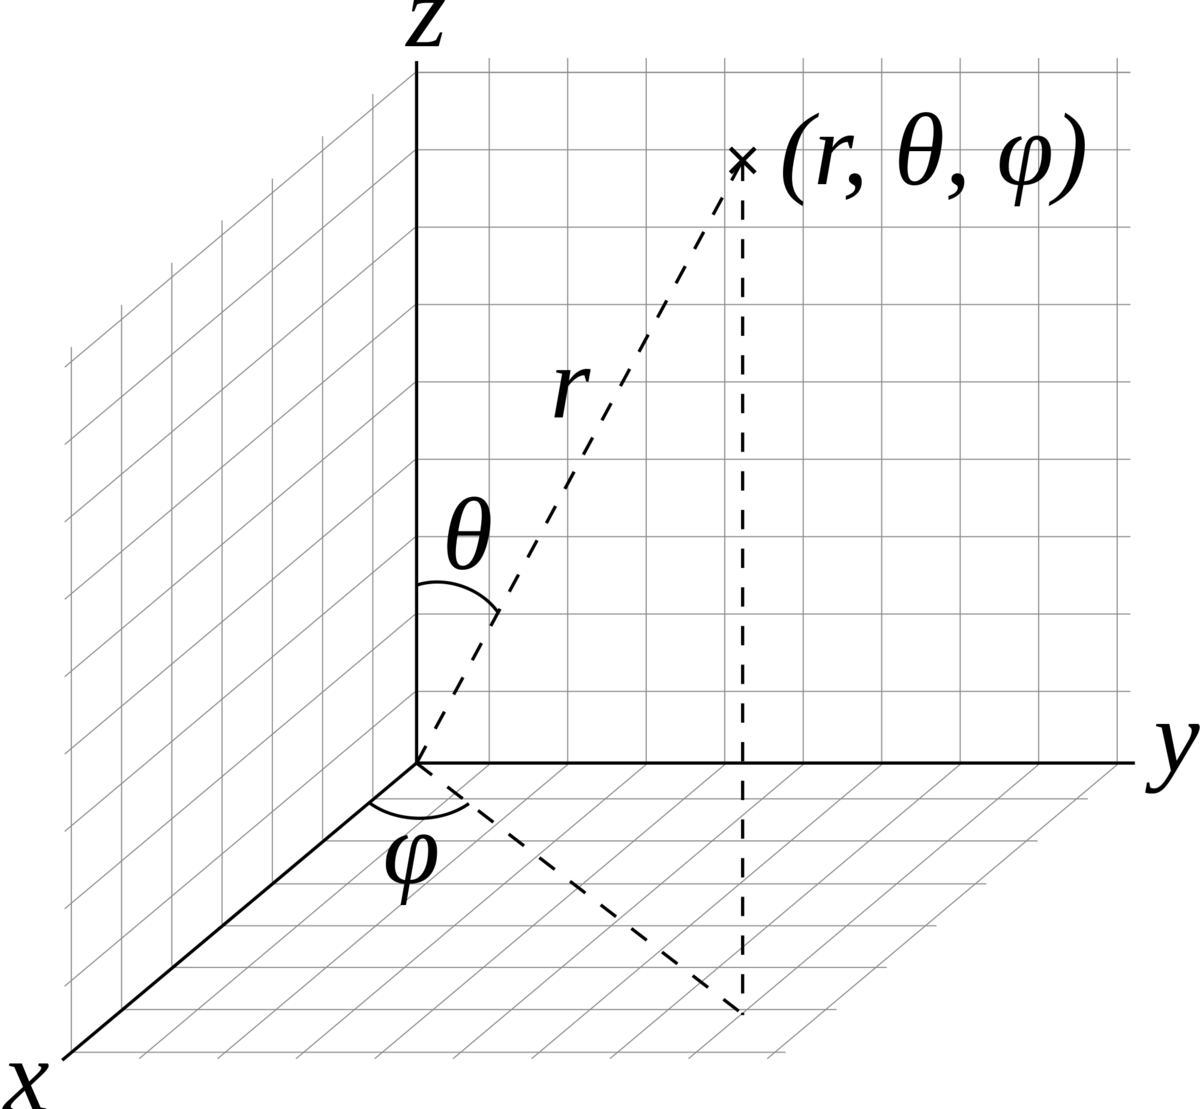
\includegraphics[width=3cm]{images/sphcoord}
\end{center}

Let us consider the first layer, i.e. the first $2l+1$ lines of 
$f_l^m$ coefficients. Then the signal can be computed 
anywhere on a point of this shell with coordinates $\theta,\phi$ as follows:
\[
f(\theta,\phi) = \sum_{l=0}^m \sum_{m=-l}^{m=+l} f_l^m Y_{lm}(\theta,\phi)
\]
with\footnote{On Wikipedia the 1st and 3rd equations are multiplied by $\sqrt{2}$ ? This make comes from 
some normalisations that include a $1+\delta_{l0}$ term in the denominator next to $4\pi$ ...?}
\begin{equation}
Y_{lm}
=
\left\{
\begin{array}{cc}
(-1)^m  {\cal I}m(Y_l^{|m|})  \propto \sin(m\phi) & m<0 \\
Y_{l,0} & m=0 \\
(-1)^m  {\cal R}e(Y_l^{m}) \propto \cos(m\phi)   & m<0 
\end{array}
\right.
\end{equation}
and
\begin{equation}
Y_l^m = \sqrt{\frac{2l+1}{4\pi}\frac{(l-m)!}{(l+m)!}} e^{im \phi} P_l^m (\cos\theta)
\label{f85:spheq}
\end{equation}
where 
$\theta$ is the colatitude ($0\le\theta\le \pi$ from North pole to South pole), $\phi$
is the longitude ($0\le\phi\le 2\pi$) and $P_l^m$ are associated Legendre polynomials. \index{general}{Legendre Polynomials} Note that $Y_{lm}$ is a real number while $Y_l^m$ is a complex number.

The first few lines of {\sl S20RTS.sph} are shown hereunder:
\begin{tiny}
\begin{verbatim}
             20 111111111111111111111  24 000111111111111111111111 
  0.1534E-01
  0.1590E-01 -0.1336E-01  0.3469E-02
 -0.3480E-02  0.1165E-01  0.8376E-02  0.2158E-01 -0.9923E-02
 -0.1301E-02 -0.5792E-02  0.1049E-02 -0.7702E-02  0.1281E-02  0.1419E-01  0.8916E-02
  0.1353E-02 -0.5517E-02 -0.1429E-02 -0.1105E-01 -0.1247E-02  0.4788E-02 -0.8670E-03 -0.2317E-03  0.3142E-01
 -0.7365E-02 -0.1193E-01 -0.4838E-02 -0.1277E-01  0.1034E-03  0.6585E-02 -0.1351E-01  0.2126E-01 -0.1926E-01 -0.4675E-02 -0.7870E-02
  0.5379E-02  0.7332E-02  0.9048E-02 -0.7672E-02  0.1306E-01 -0.2900E-02 -0.1380E-01 -0.2366E-02  0.7911E-02 -0.9940E-02 -0.1281E-02  0.1321E-02 -0.1439E-02
\end{verbatim}
\end{tiny}

We see that the first line (after the header) contains one coefficient, corresponding to ${l=0},{m=0}$. 
The second line contains three coefficients which correspond to ${l=1},{m=-1,0,1}$. The third line contains 5 
coefficients, the fourth 7, etc ... 
In the case of S20RTS this goes on until $l=20$ and the line therefore contains 41 coefficients.
In the case of S40RTS this goes on until $l=40$ and the line contains 81 coefficients.
Unfortunately only 11 numbers are stored on a single line so the 81 coeffs corresponding to $l=40$ 
are spread across many lines, which makes read in the file a bit of nightmare. 
Both models are composed of 21 concentric layers so the above structure is repeated 21 times in the files. 
The structure of the file is explained in the ASPECT manual (but it remains a mystery as to where this information comes from ...) in a cookbook authored by Jacqueline Austermann:  
"The first number in the first line denotes the maximum degree. This is followed in
the next line by the spherical harmonic coefficients from the surface down to the
CMB. The coefficients are arranged in the following way:\\

\noindent $a_{00}$ \\
$a_{10}$ $a_{11}$ $b_{11}$ \\
$a_{20}$ $a_{21}$ $b_{21}$ $a_{22}$ $b_{22}$ \\
... \\

$a_{lm}$ is the cosine coefficient of degree $l$ and order $m$; $b_{lm}$ is
the sine coefficient of degree $l$ and order $m$. 
This means that $f_l^m=a_{lm}$ when $m\ge 0$ and $f_l^m=b_{lm}$ when $m<0$."

The code uses the {\sl scipy.special.sph\_harm} function which is documented 
at \url{https://docs.scipy.org/doc/scipy/reference/generated/scipy.special.sph_harm.html}
and which implements Eq.~\eqref{f85:spheq}.

We can first focus on the first 'pyramid' of coefficients corresponding to the shell 
of zero depth and compute the seismic velocity anomaly $\delta v/v$ on a longitude/latitude
map for both S20RTS and S40RTS and compare our results with those of SubMachine \cite{homs18}.

\begin{center}
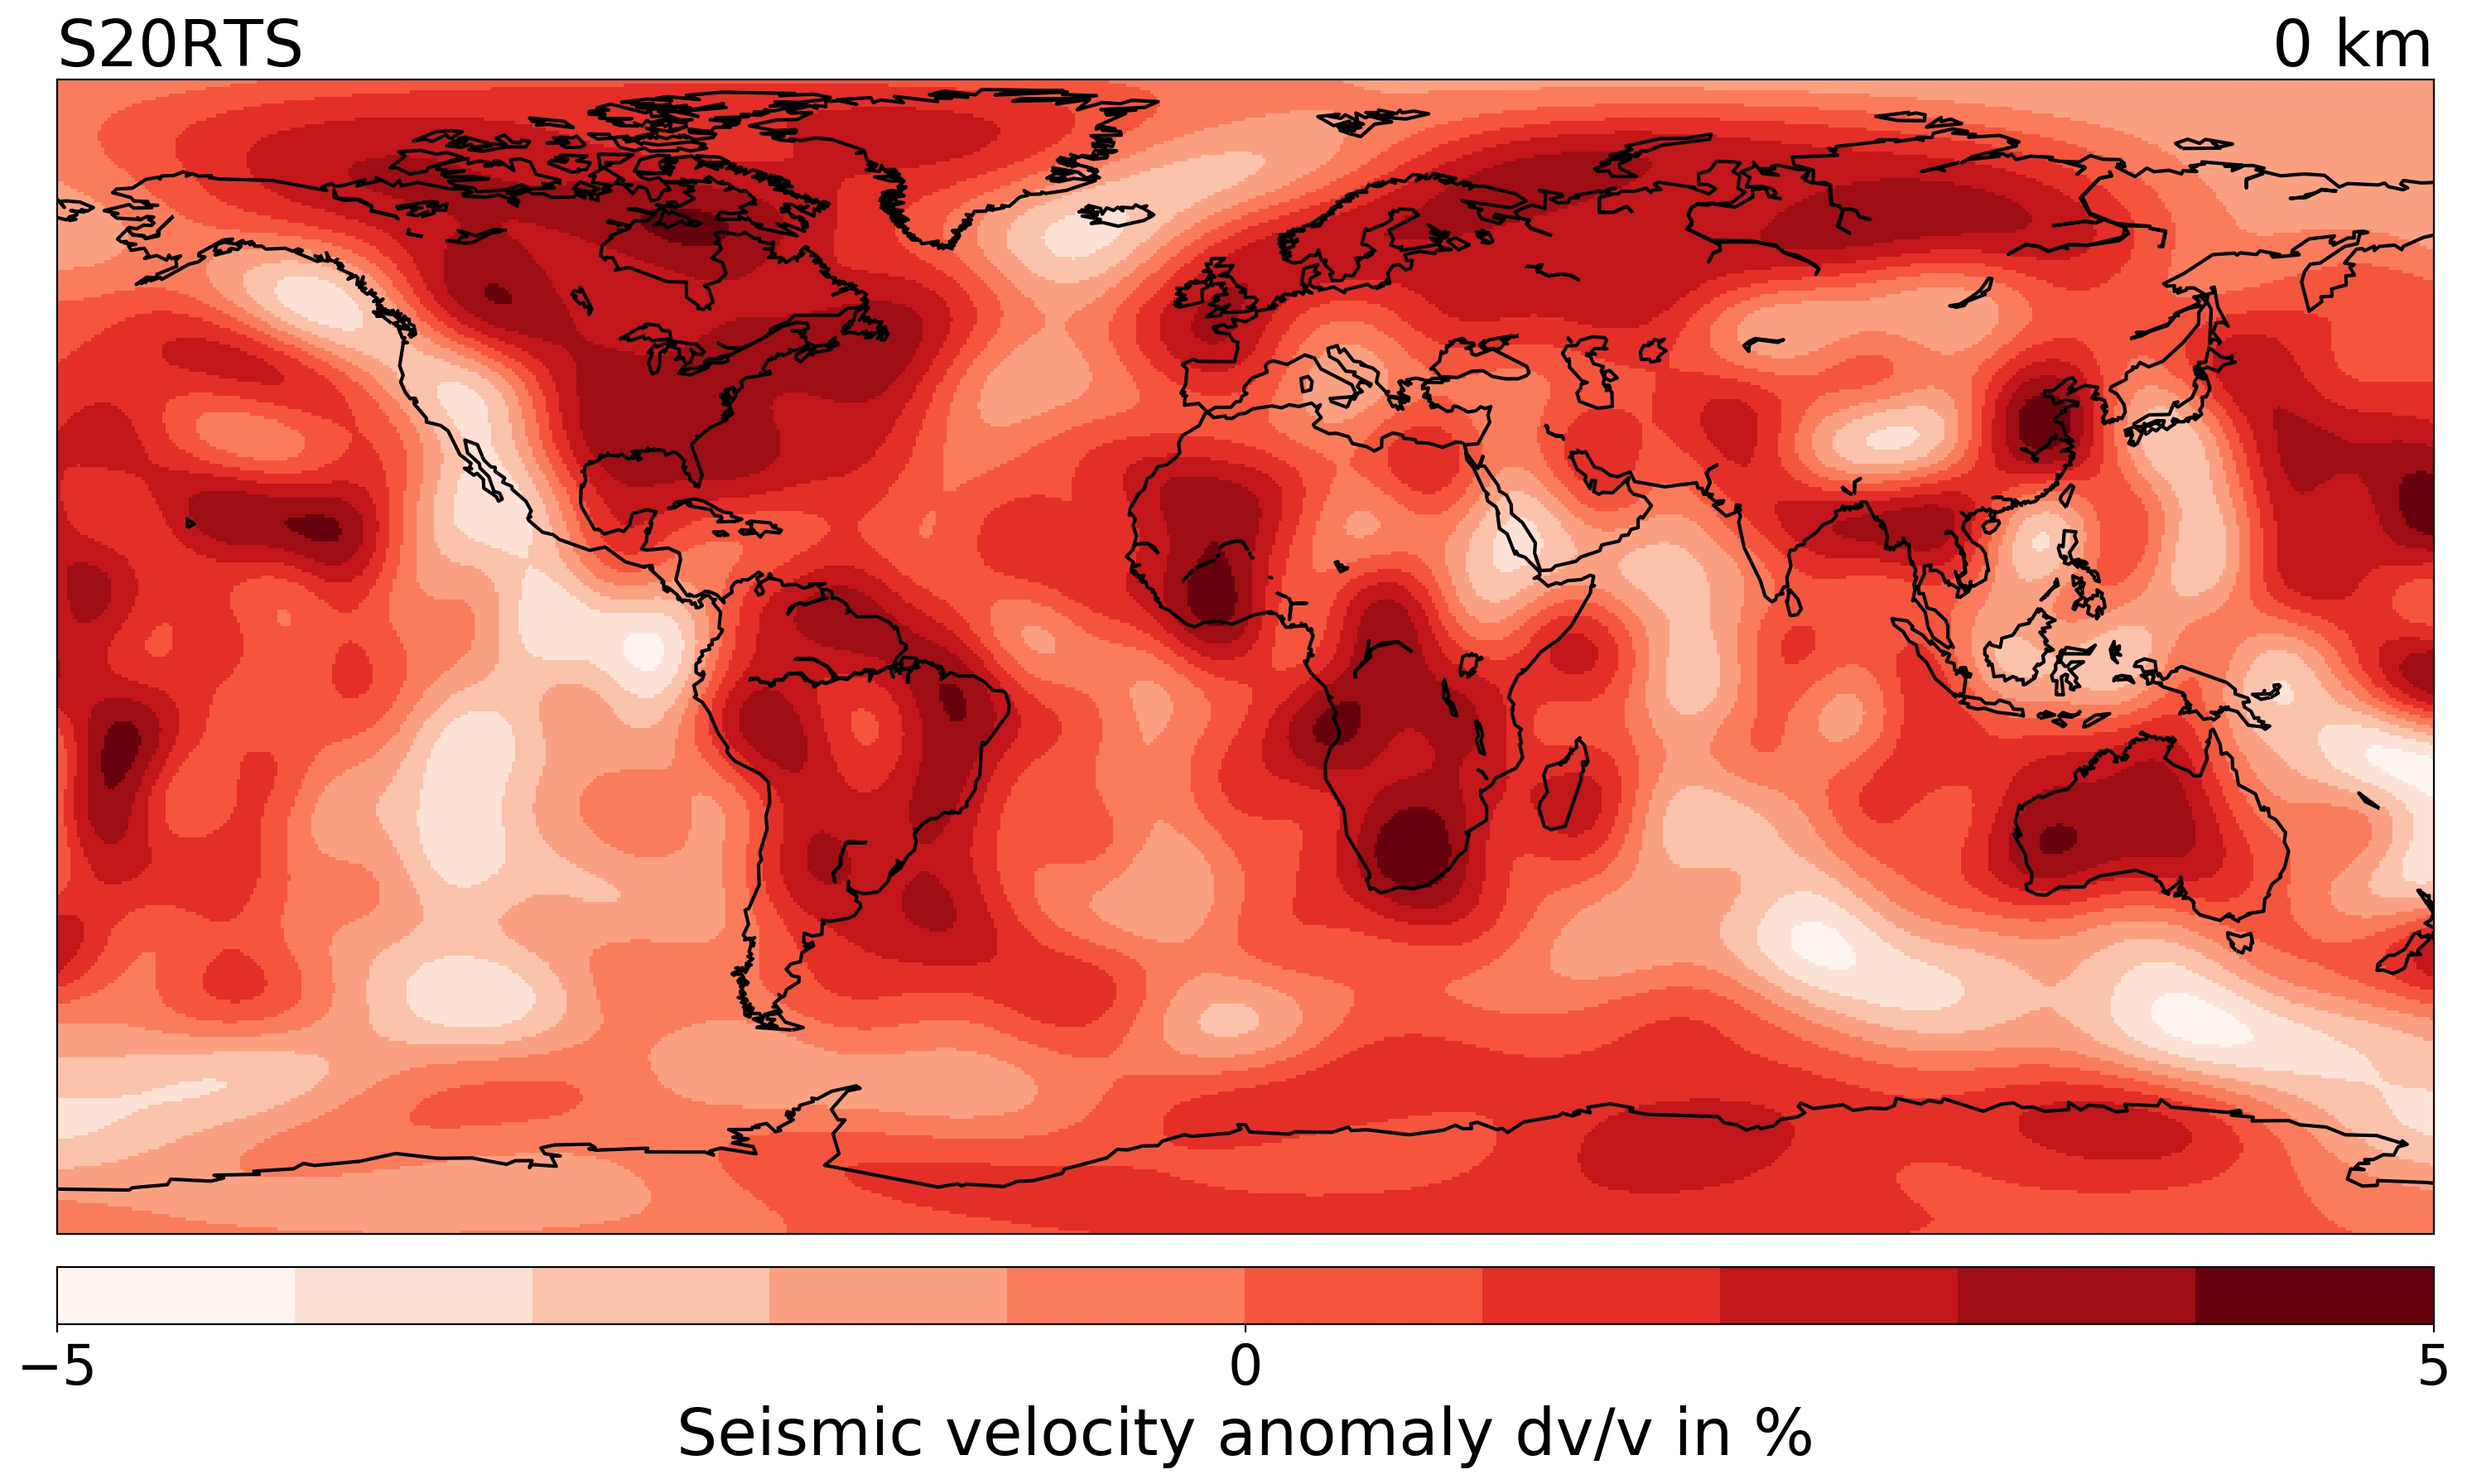
\includegraphics[width=8cm]{python_codes/fieldstone_85/S20}
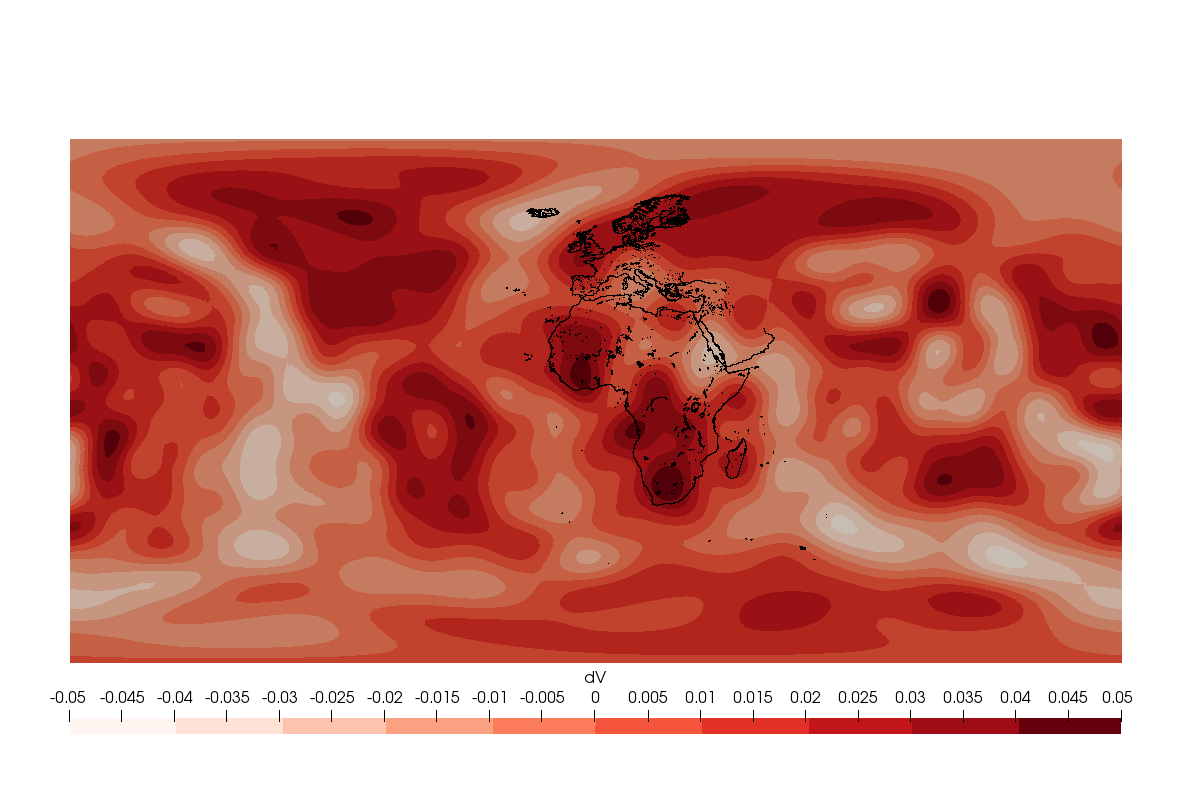
\includegraphics[width=8cm]{python_codes/fieldstone_85/S20mine}\\
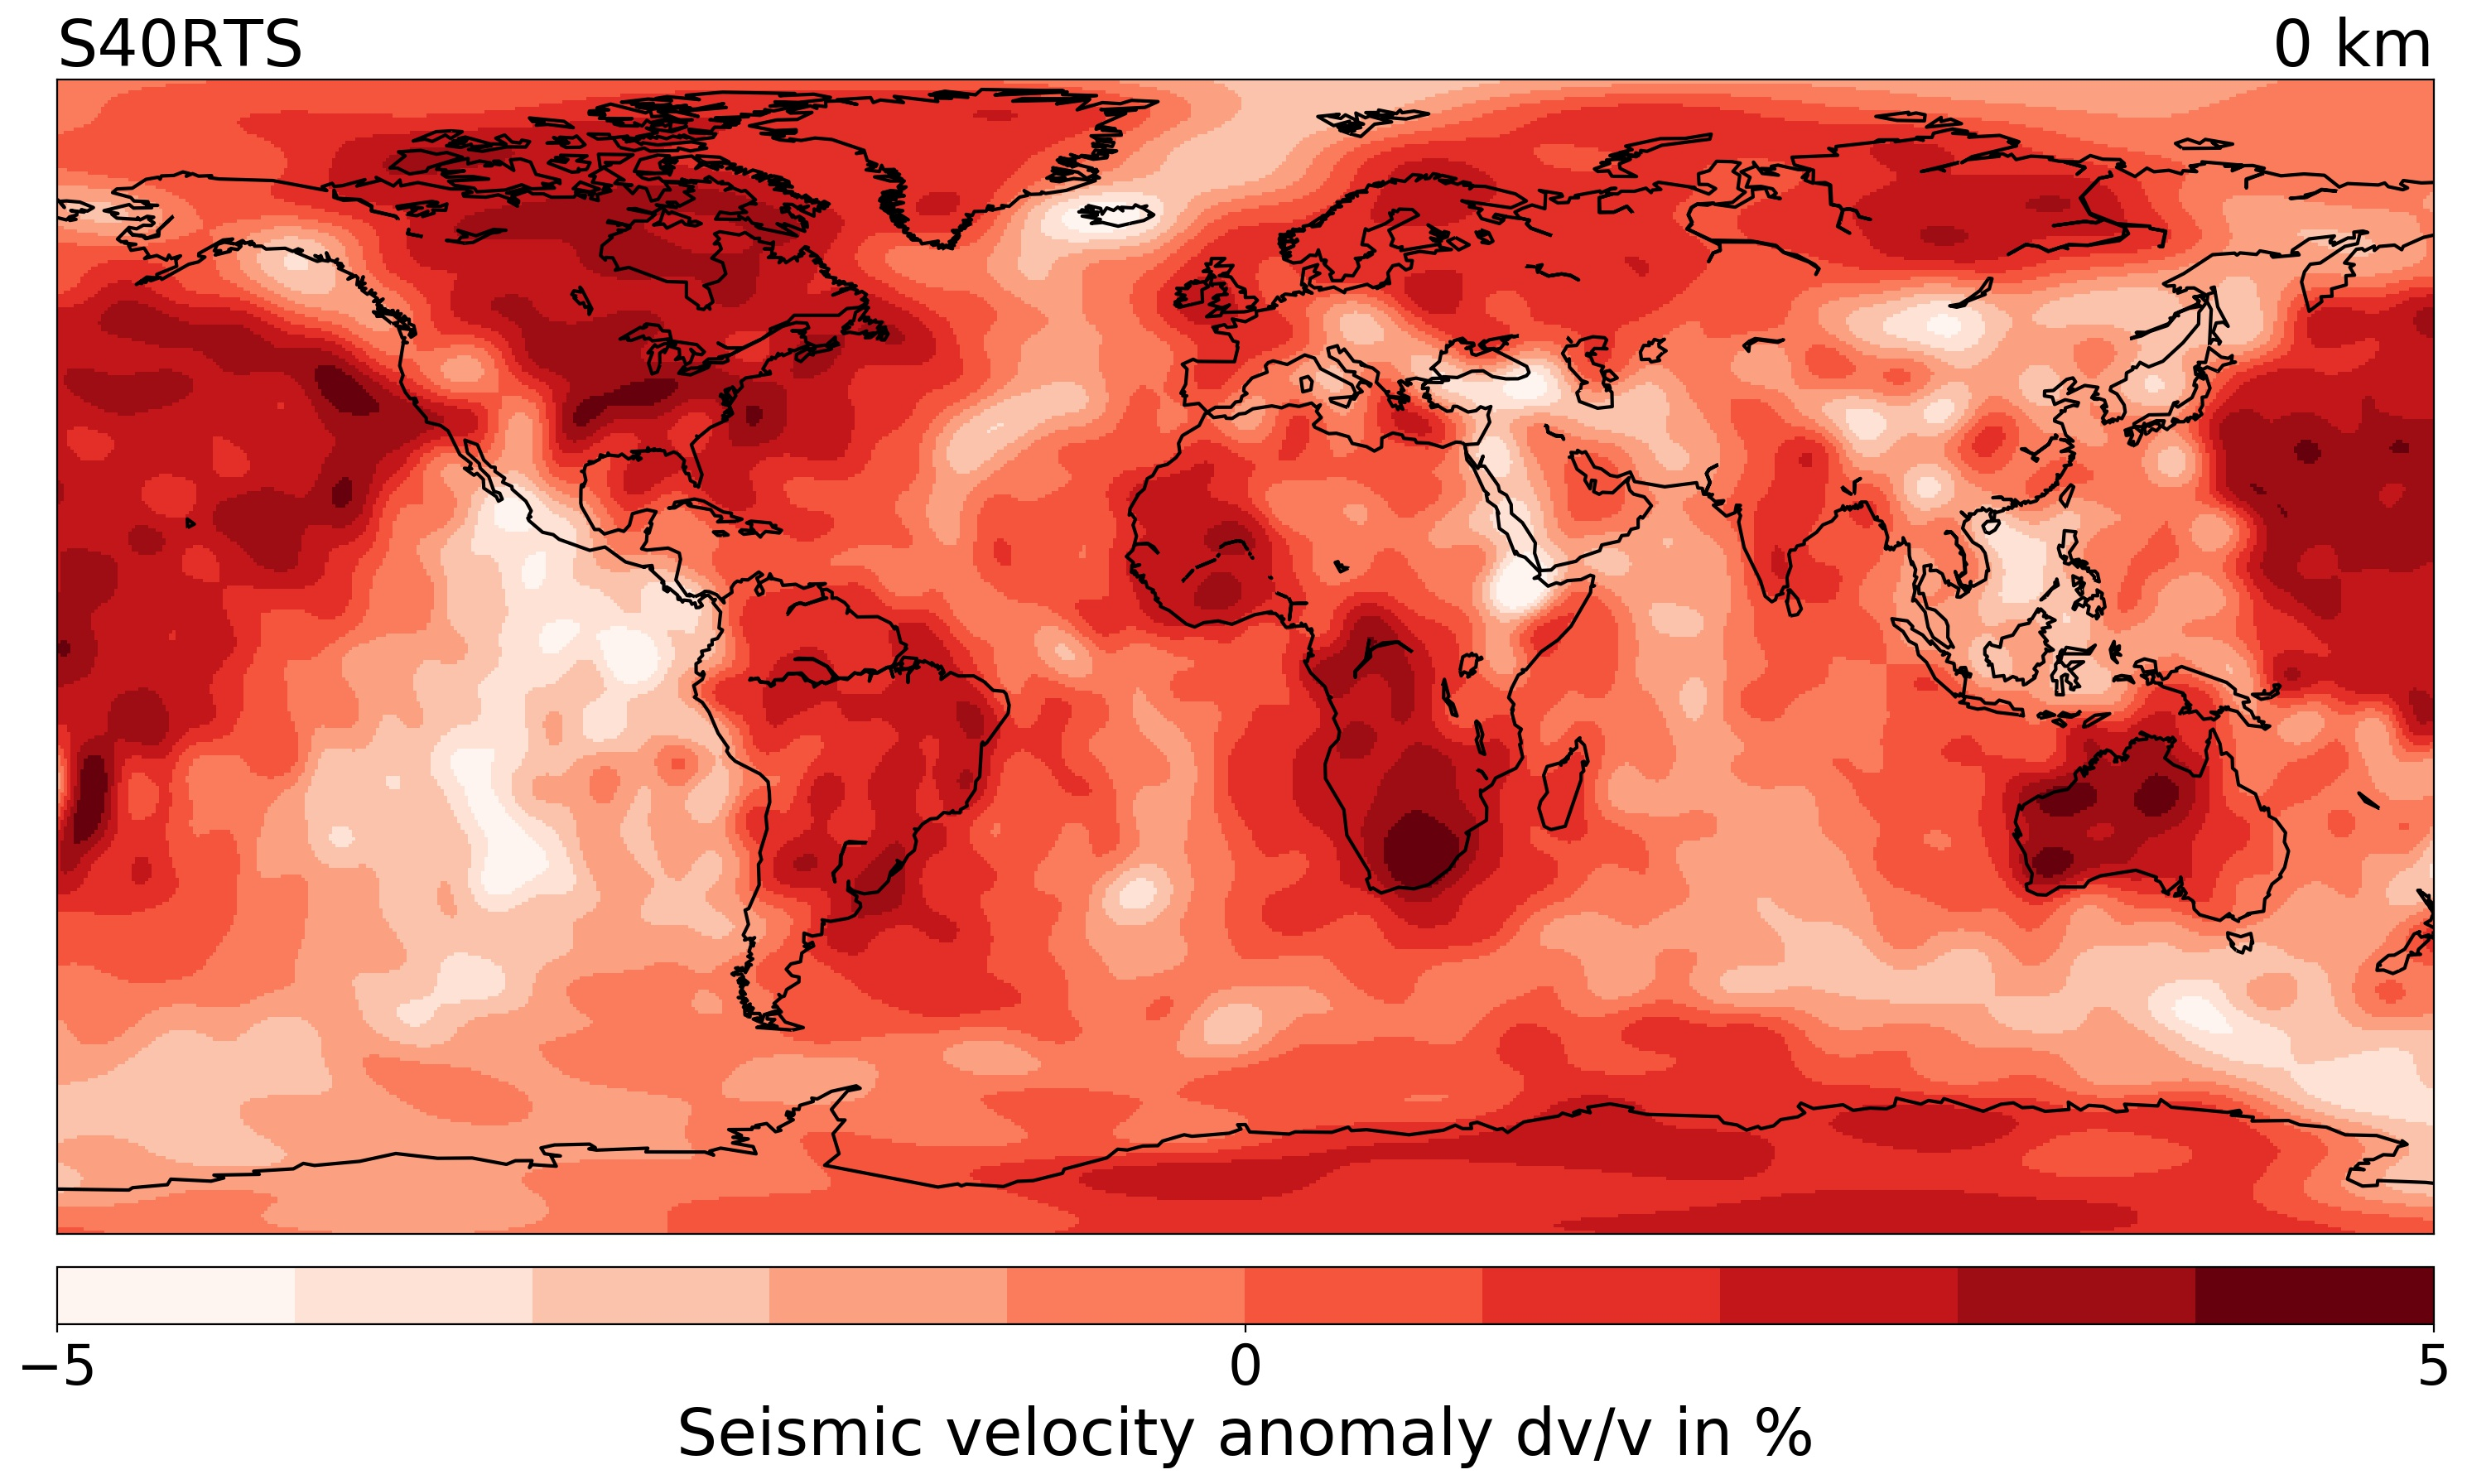
\includegraphics[width=8cm]{python_codes/fieldstone_85/S40}
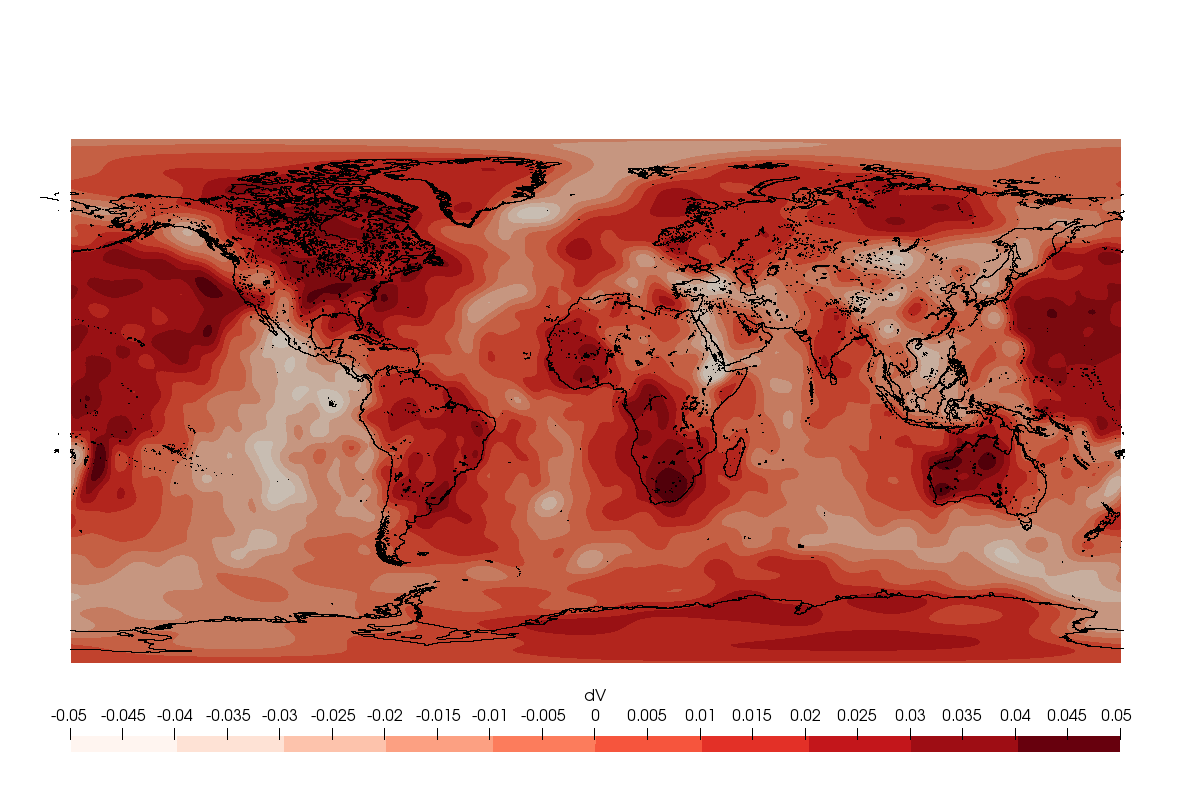
\includegraphics[width=8cm]{python_codes/fieldstone_85/S40mine}\\
{\captionfont Comparison between Submachine (left) and this stone (right) at 0 depth.
The vtu files for the coastlines are obtained by running Stone~69.}
\end{center}

\begin{center}
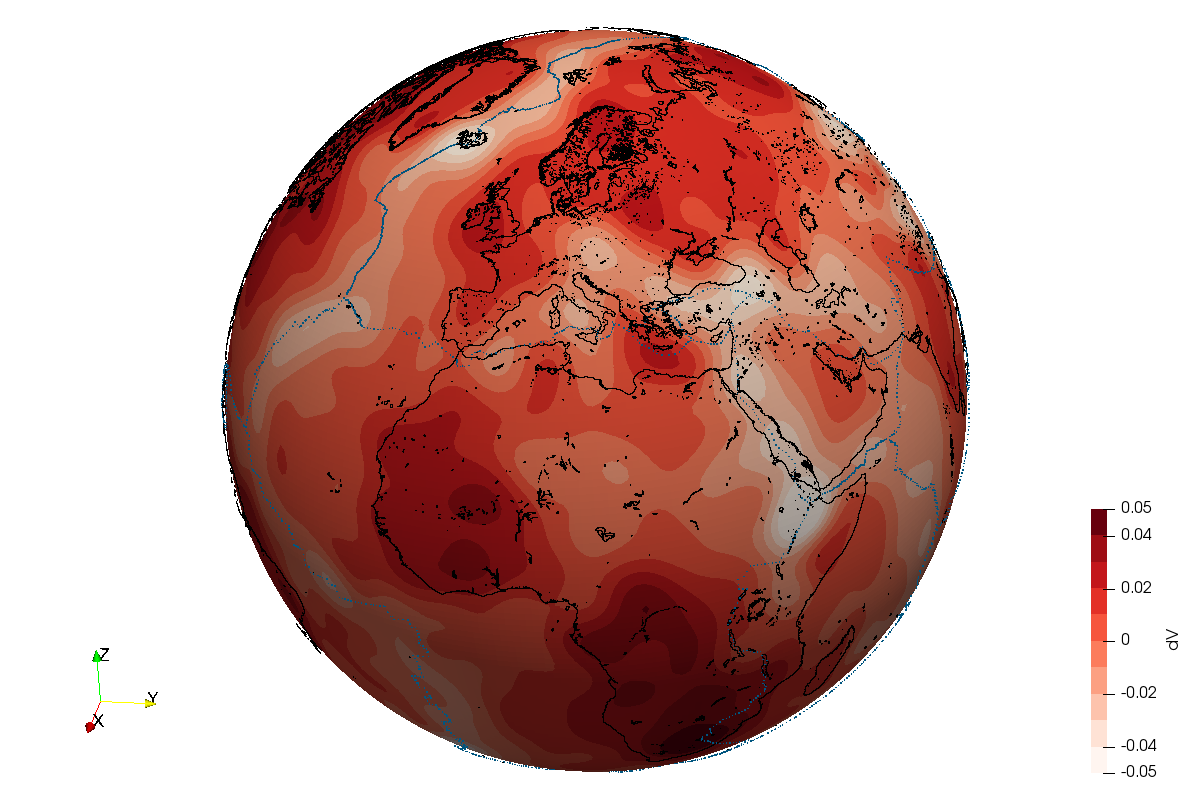
\includegraphics[width=5.2cm]{python_codes/fieldstone_85/S40mine_sphere1}
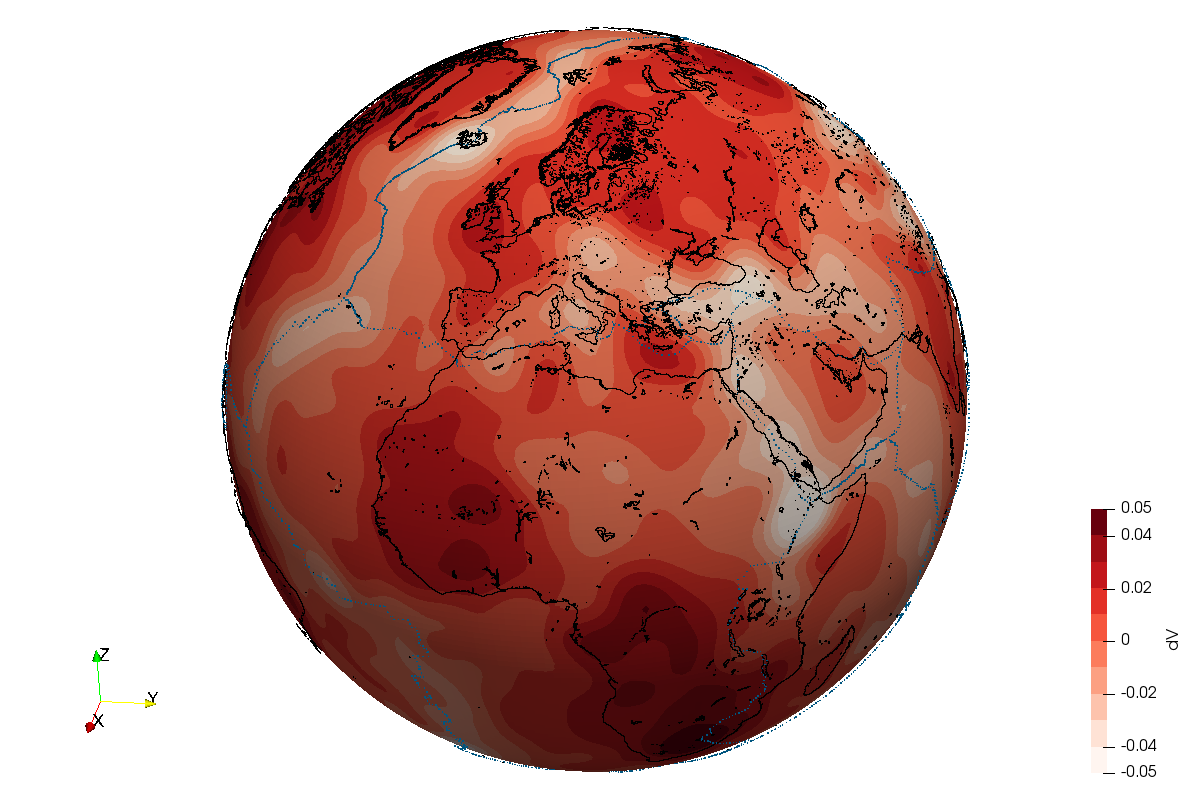
\includegraphics[width=5.2cm]{python_codes/fieldstone_85/S40mine_sphere1}
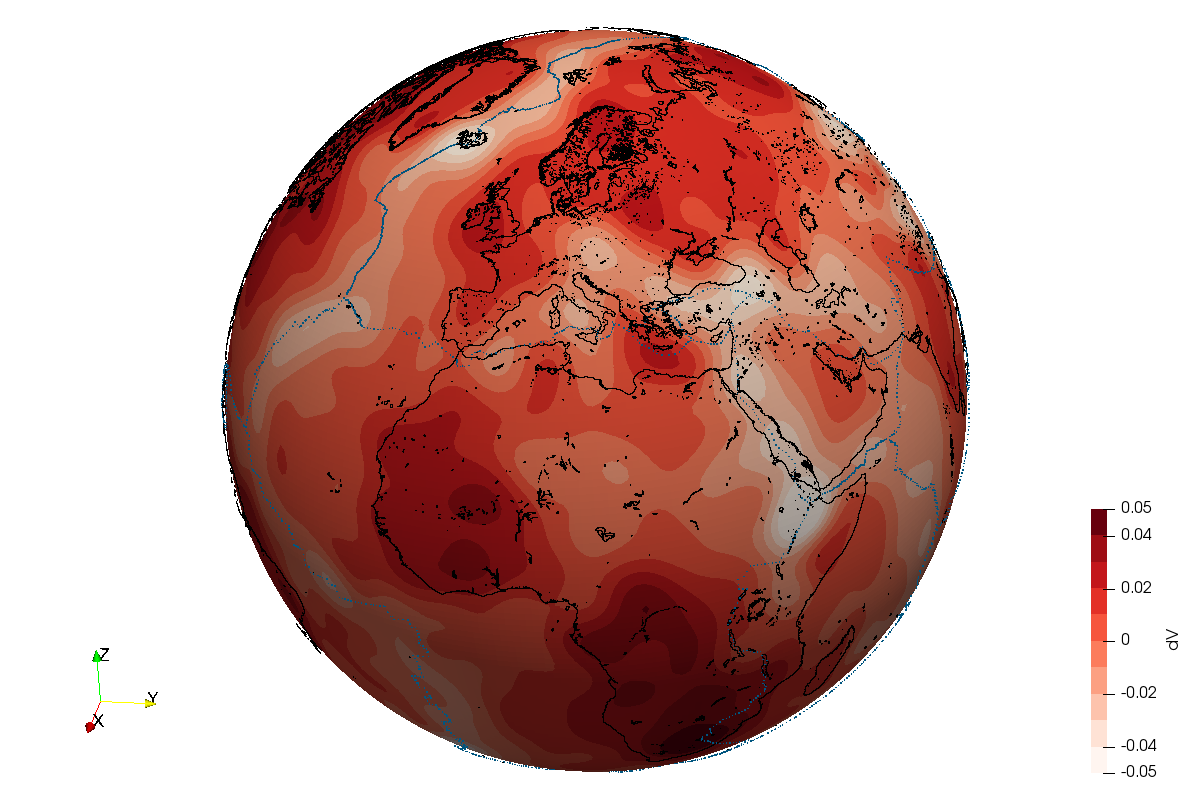
\includegraphics[width=5.2cm]{python_codes/fieldstone_85/S40mine_sphere1}\\
{\captionfont Seismic velocity anomaly, 0 depth, S40RTS.}
\end{center}


COMPARE WITH ORIGINAL RITSEMA PROGRAM





Of course, one may wish to compute $f$ at a value of $r$ that does not coincide with one of the 21 layers... 
and this is where spline functions come in.  
In Ritsema et al \cite{ridv11}, one reads: "We use the same 
spline functions as in Ritsema et al (2004) \cite{rivw04} to parametrize vertical 
variation of shear velocity. The separation of the spline functions
increases with depth. Relatively dense spline distribution helps to
accommodate strong vertical shear-velocity variations across the
lithosphere–asthenosphere boundary and the phase transition in the
transition zone albeit at the expense of the vertical resolution at
the base of the mantle."
Unfortunately the 2004 paper does not reveal the values of the spline knots, but the values
are available in the {\sl splhsetup.f} file included in the tools available 
on J. Ritsema's website \url{https://jritsema.earth.lsa.umich.edu/Research.html}.


\begin{center}
\begin{tabular}{cccl}
\hline 
normalised & radius & depth & spline number\\
\hline 
\hline 
1.00000  & 2891.        &  0            & 0 (surface)\\
0.96512  & 2840.58096   &  50.41904     & 1\\
0.92675  & 2785.117125  &  105.882875   & 2\\
0.88454  & 2724.10257   &  166.89743    & 3\\
0.83810  & 2656.97355   &  234.02645    & 4\\
0.78701  & 2583.122955  &  307.877045   & 5\\
0.73081  & 2501.885855  &  389.114145   & 6\\
0.66899  & 2412.525045  &  478.474955   & 7\\
0.60097  & 2314.202135  &  576.797865   & 8\\
0.52615  & 2206.049825  &  684.950175   & 9\\
0.44384  & 2087.07072   &  803.92928    & 10\\
0.35329  & 1956.180695  &  934.819305   & 11\\
0.25367  & 1812.179985  &  1078.820015  & 12\\
0.14409  & 1653.782095  &  1237.217905  & 13\\
0.02353  & 1479.512615  &  1411.487385  & 14\\
-0.10909 & 1287.810405  &  1603.189595  & 15\\
-0.25499 & 1076.911955  &  1814.088045  & 16\\
-0.41550 & 844.89475    &  2046.10525   & 17\\
-0.59207 & 589.662815   &  2301.337185  & 18\\
-0.78631 & 308.888895   &  2582.111105  & 19\\
-1.00000 & 0            &  2891         & 20  (CMB) \\
\hline
\end{tabular}\\
{\captionfont Spline knots}
\end{center}

The values in the table above seem to correspond to the figure taken from 
Ritsema et al (2004) \cite{rivw04} shown hereunder. 

\begin{center}
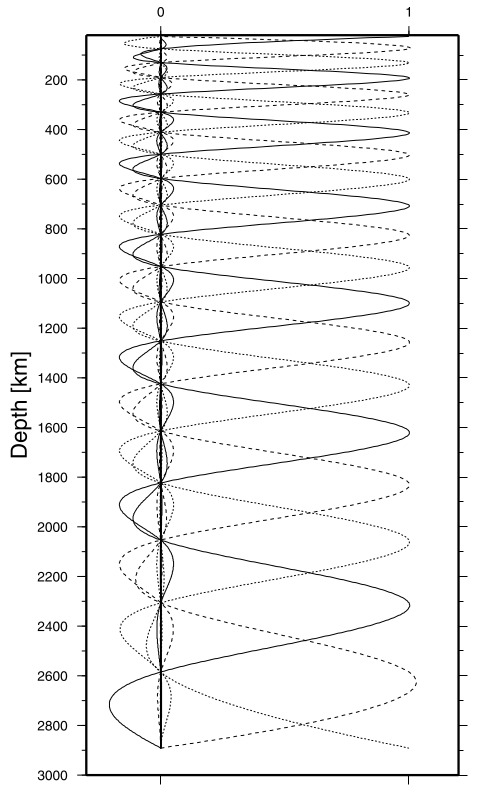
\includegraphics[width=5cm]{python_codes/fieldstone_85/rivw04splines}
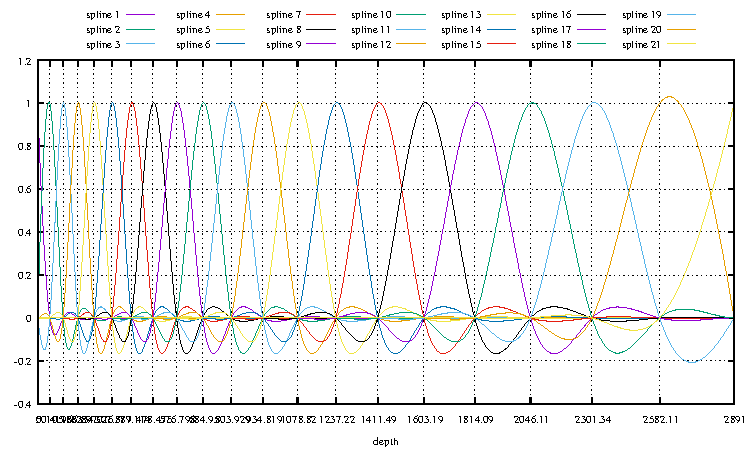
\includegraphics[width=10cm]{python_codes/fieldstone_85/splines/splines.pdf}\\
{\captionfont Left: Taken from Ritsema et al (2004) \cite{rivw04}.
Right: Data obtained from R. Maguire's code on github\footnote{\url{https://github.com/romaguir/sph_models}}.
We see that the splines are zero at the depths/nodes 
indicated by the tics on the x axis, and that 
they are 1 on their respective node, i.e. $B_i(d_j)=\delta_{ij}$}
\end{center}






\begin{center}
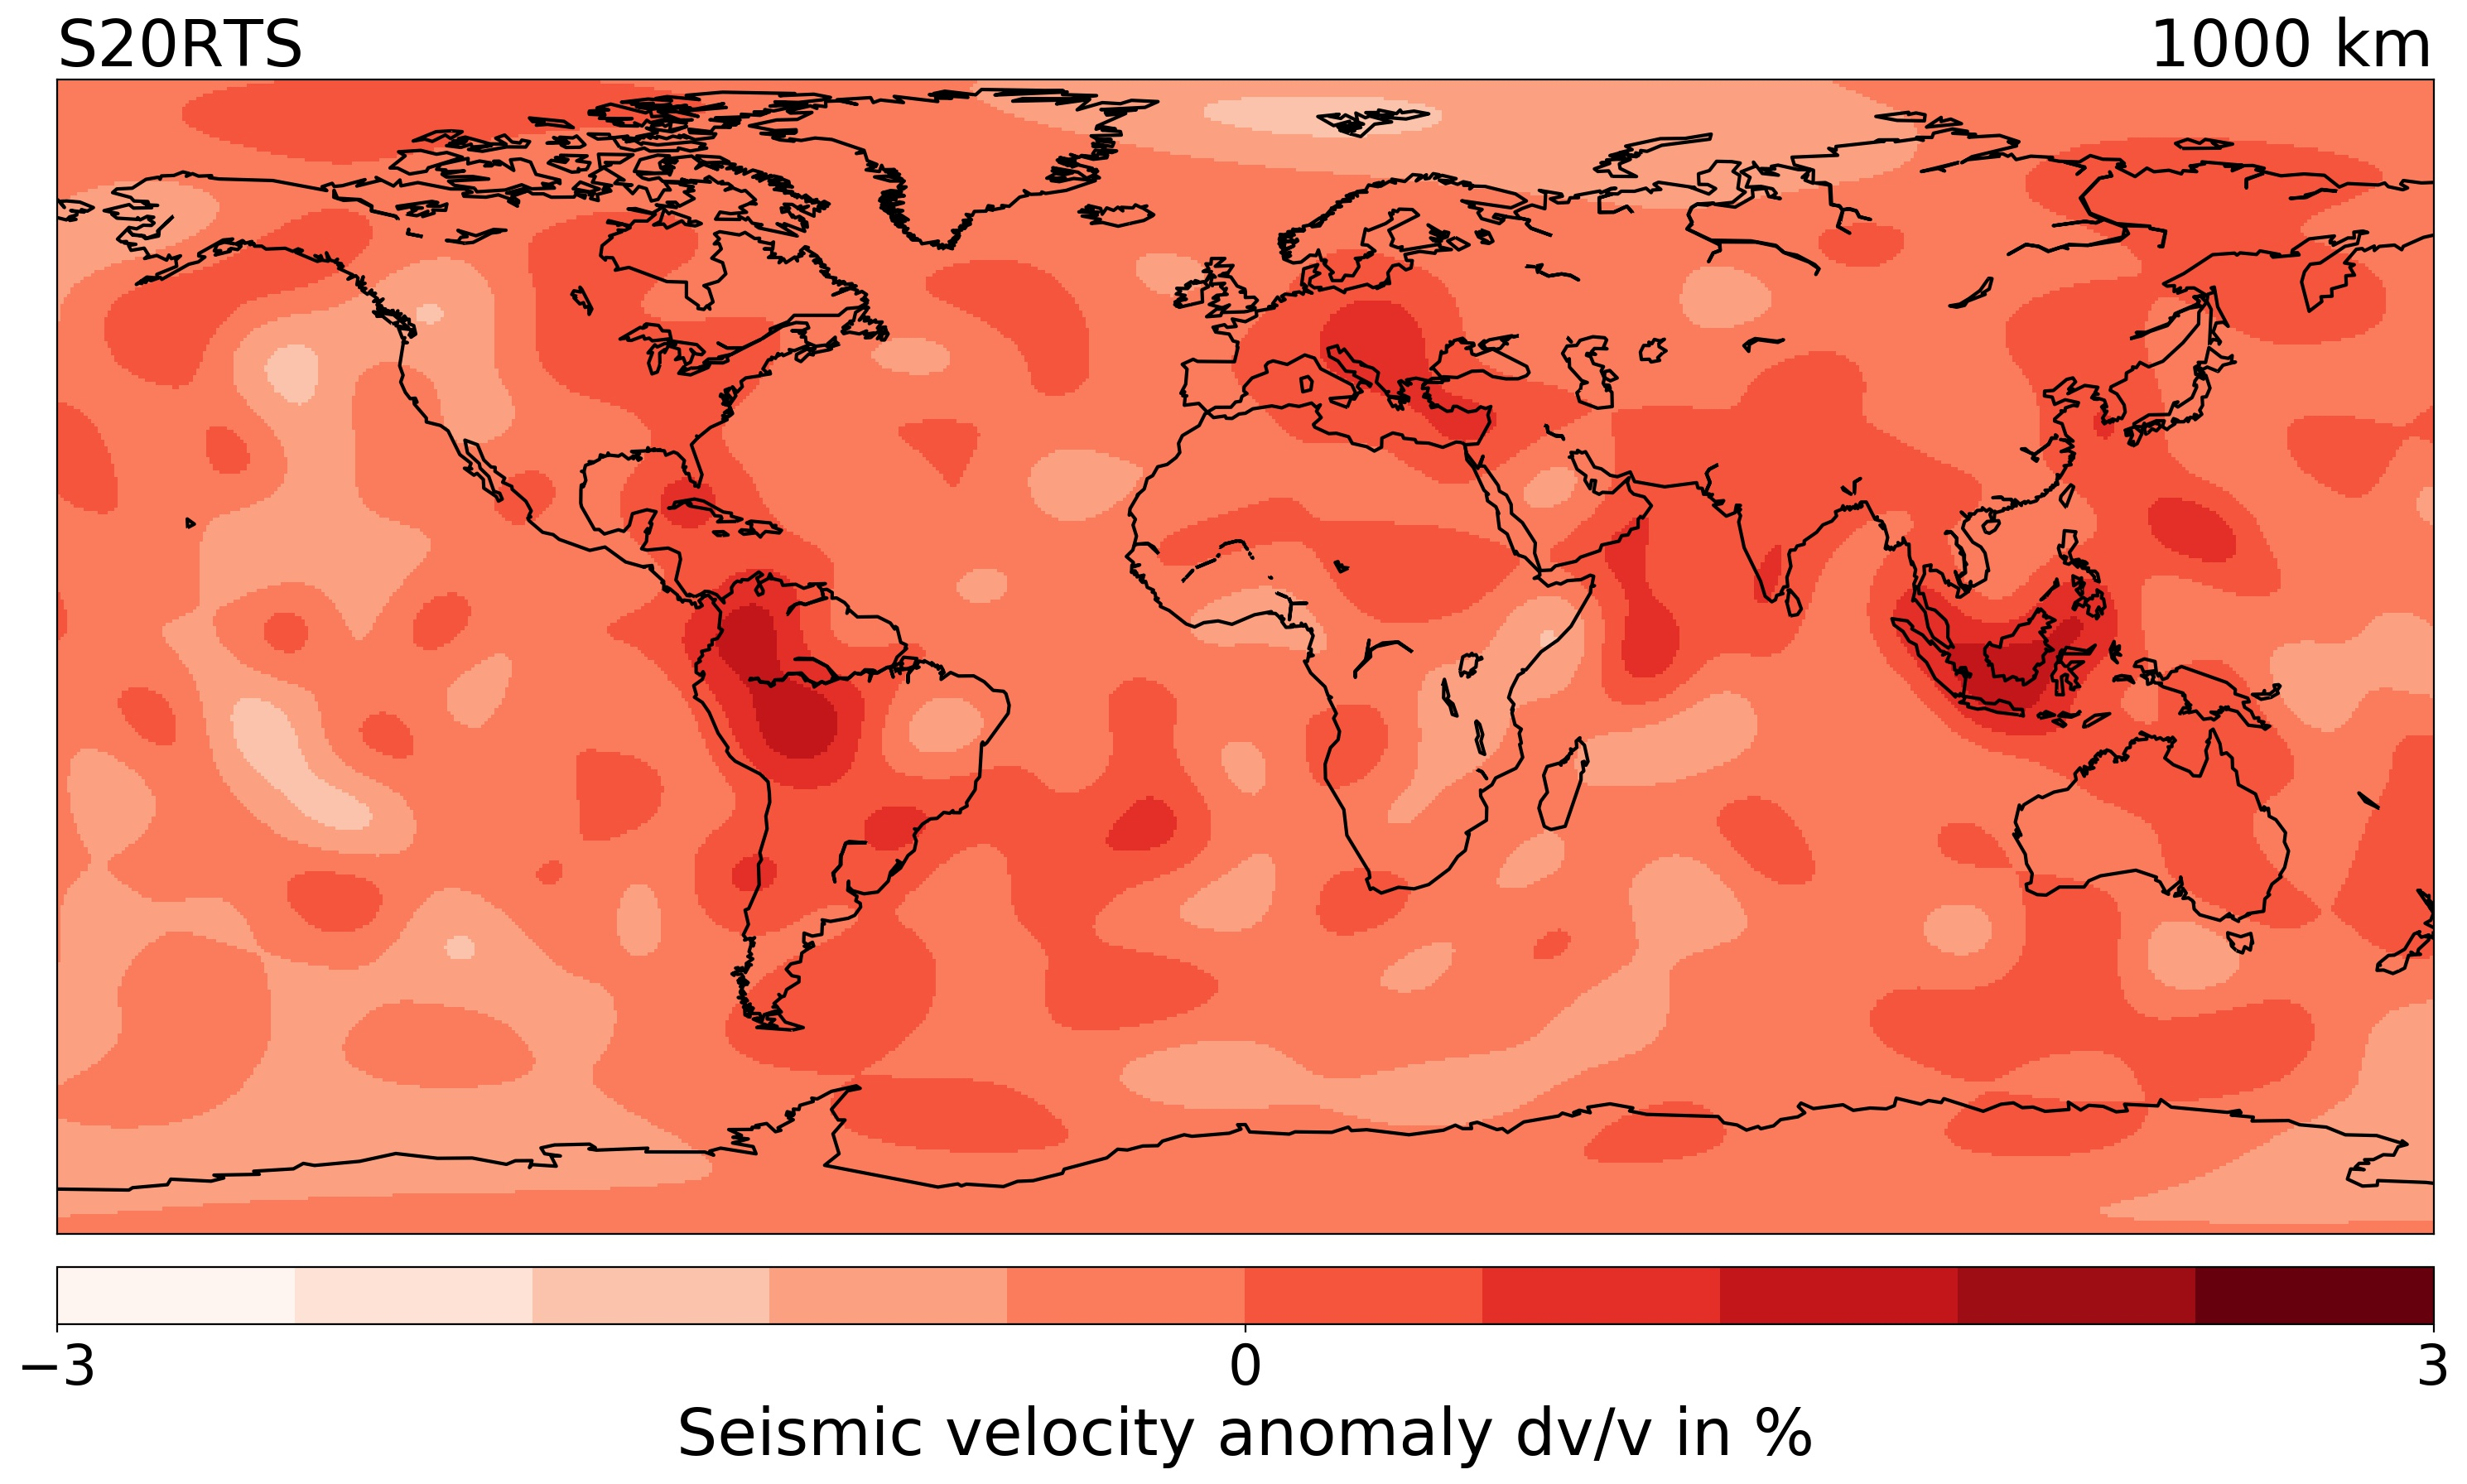
\includegraphics[width=8cm]{python_codes/fieldstone_85/S20_1000}
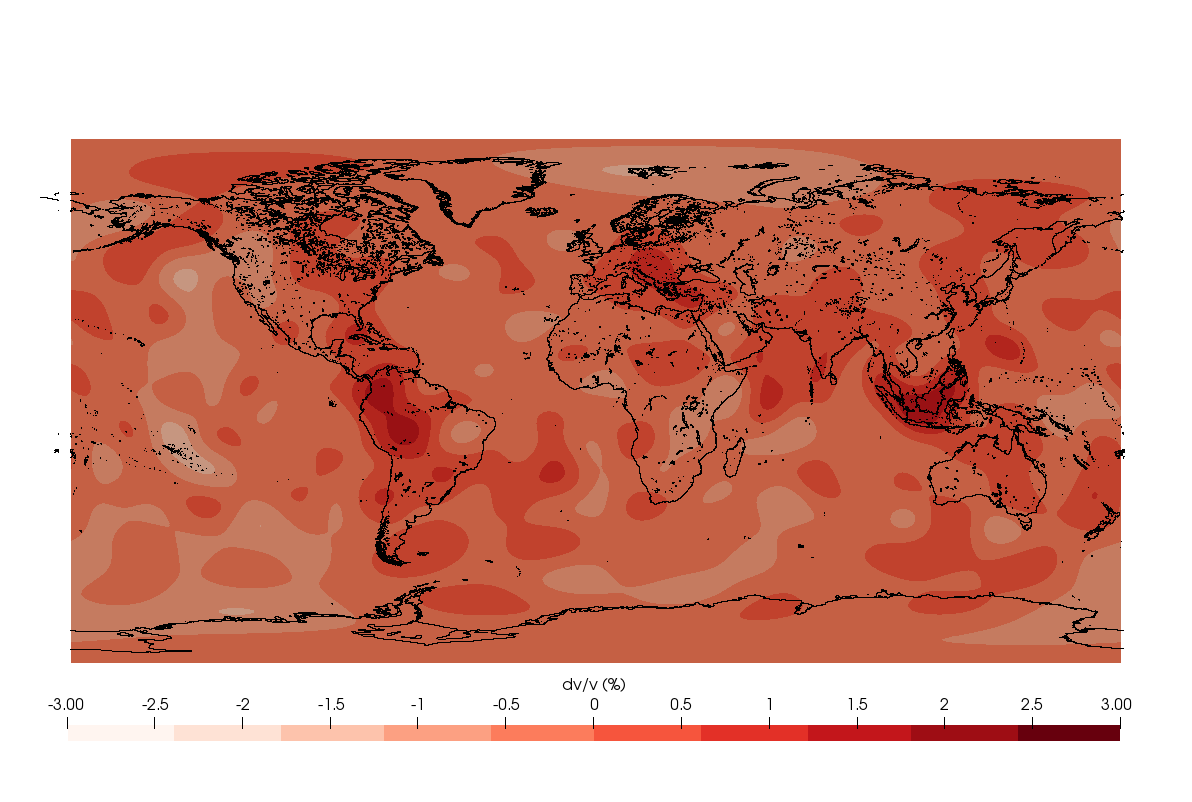
\includegraphics[width=8cm]{python_codes/fieldstone_85/S20_1000mine}\\
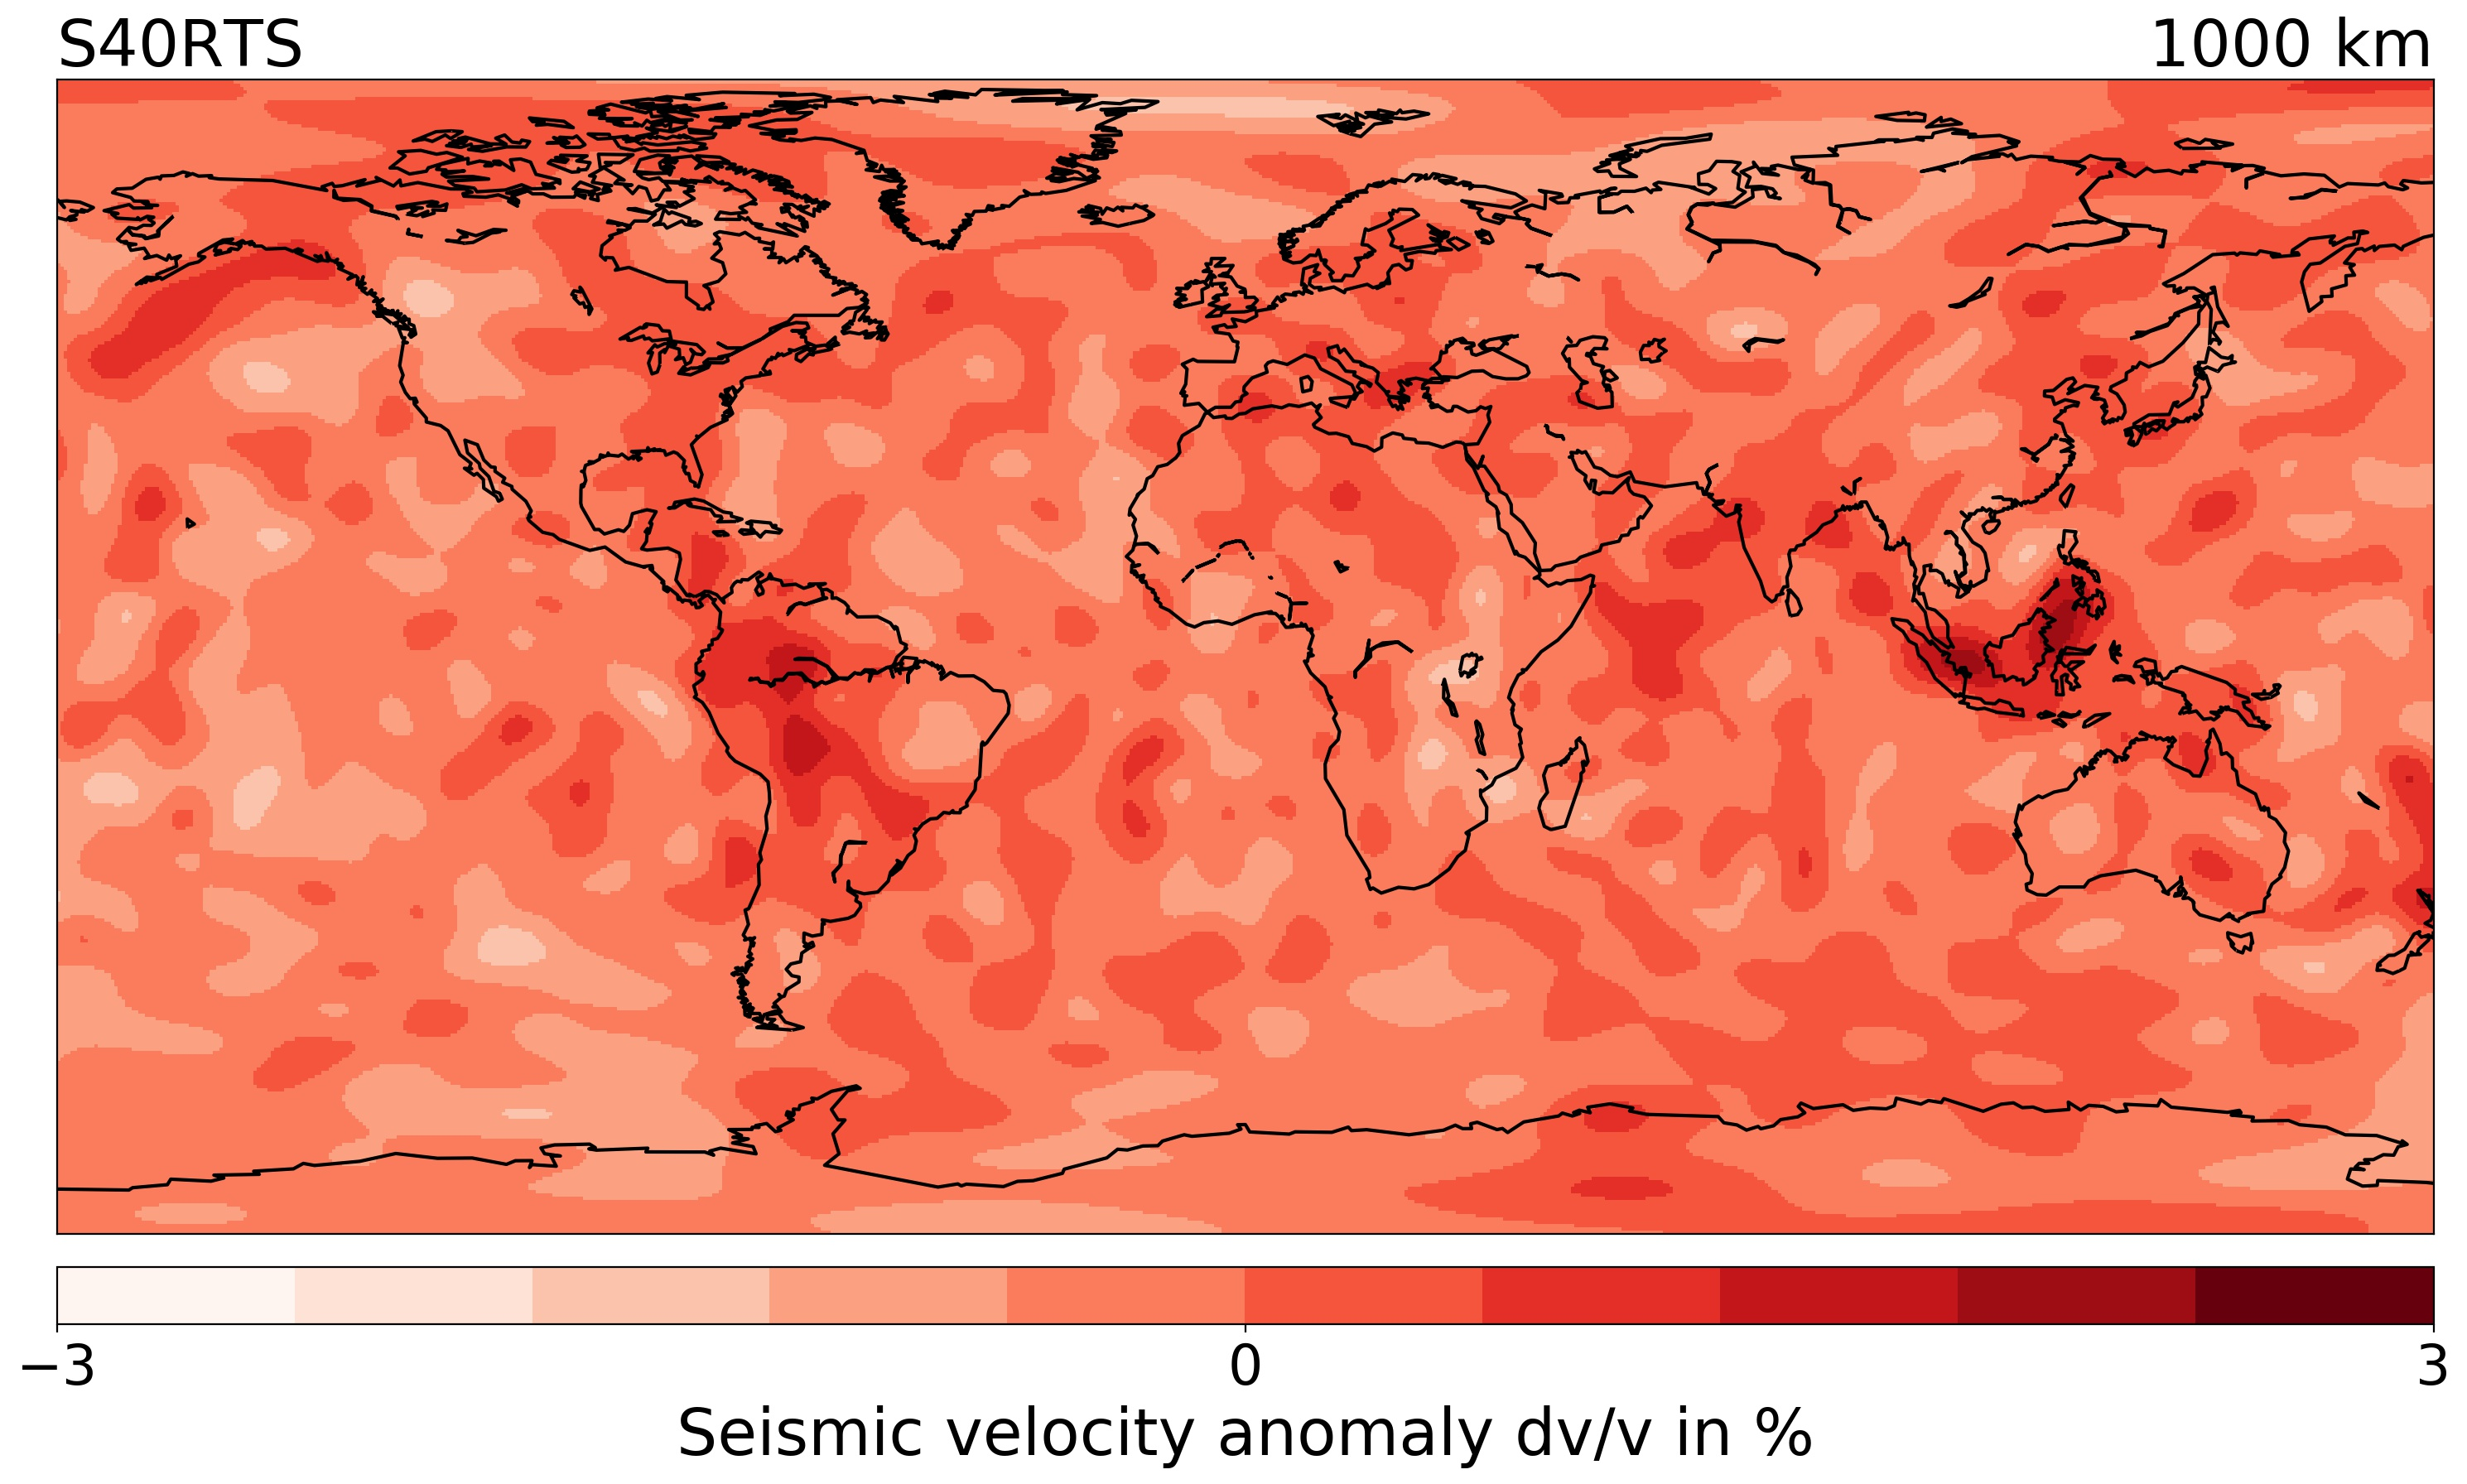
\includegraphics[width=8cm]{python_codes/fieldstone_85/S40_1000}
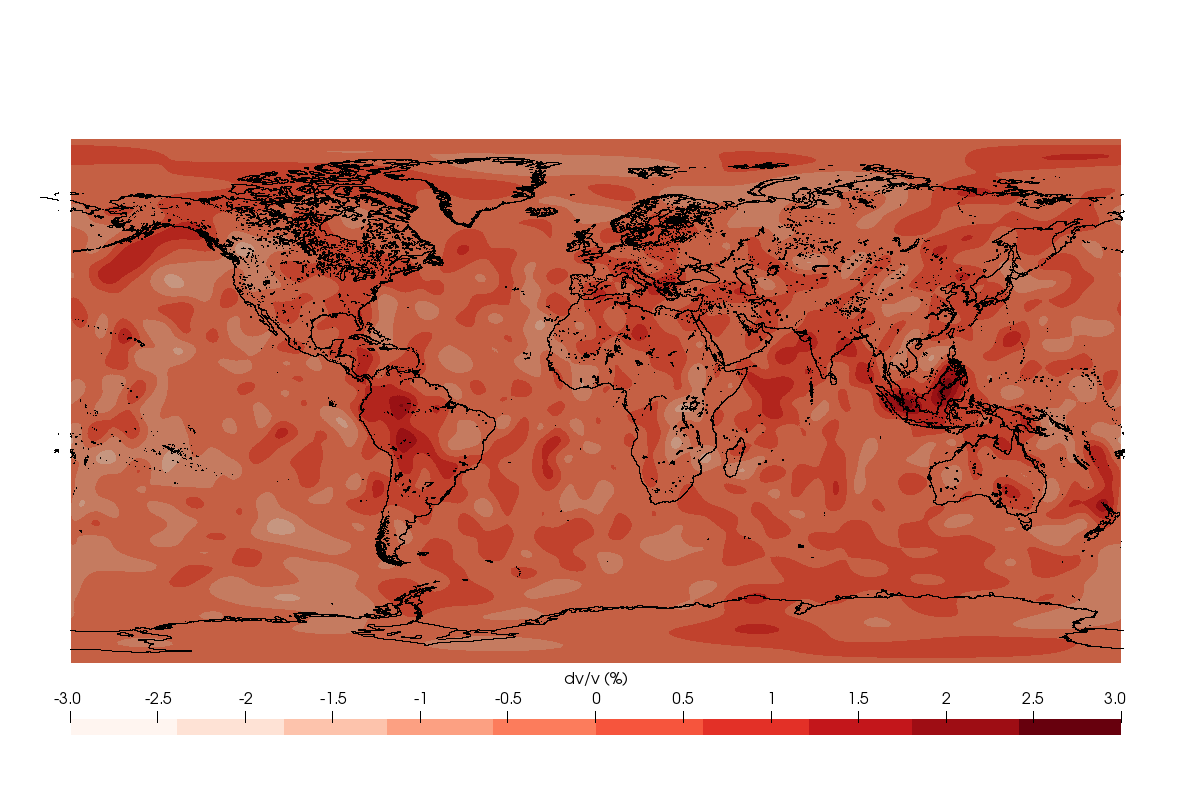
\includegraphics[width=8cm]{python_codes/fieldstone_85/S40_1000mine}\\
\end{center}



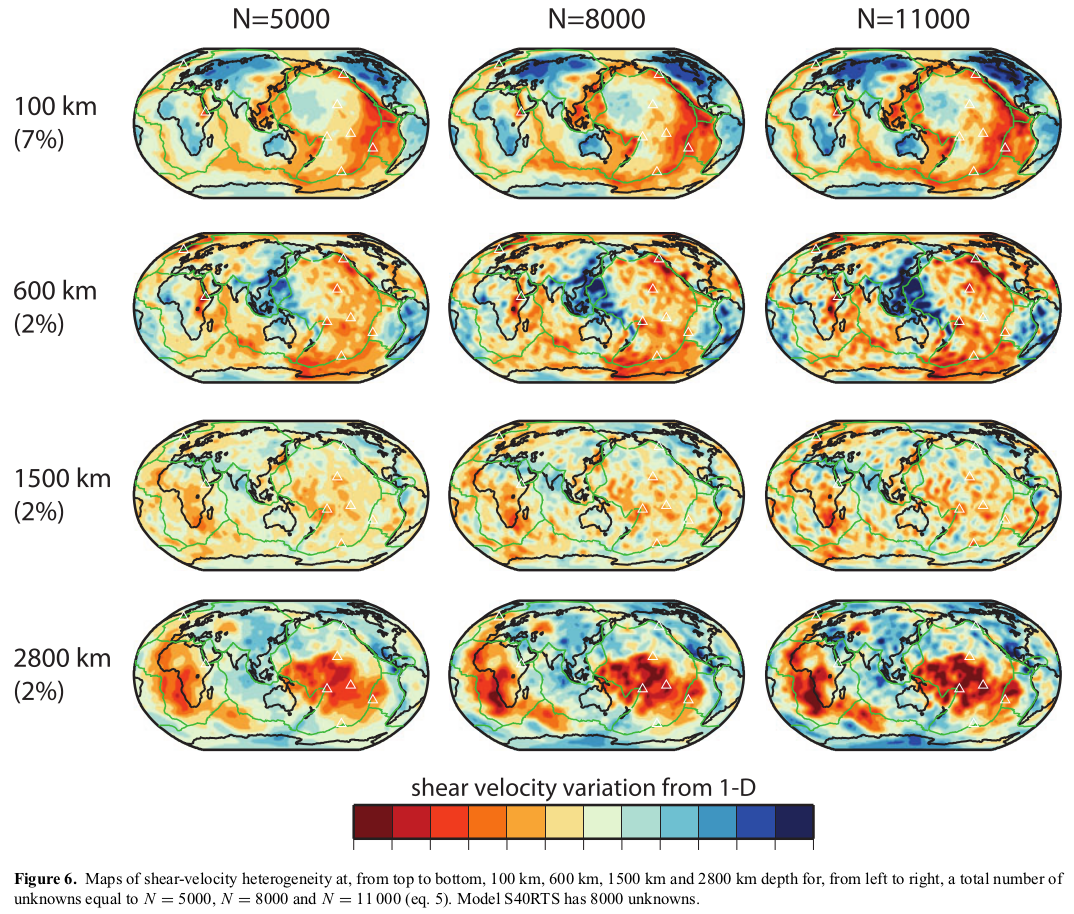
\includegraphics[width=10cm]{python_codes/fieldstone_85/ridv11}


